\documentclass{article}
% Language setting
\usepackage[english]{babel}

% Set page size and margins
\usepackage[a4paper]{geometry}

% Useful packages
\usepackage{amsmath}
\usepackage{graphicx}
\usepackage[colorlinks=true, allcolors=blue]{hyperref}

% Images
\usepackage{graphicx}
\graphicspath{ {./Images/} }

\renewcommand*\contentsname{Summary}

\title{%
  LibreSpeed C Backend Implementation \\
  \large Computer Networks Course (Prof. C. Ardagna, Prof. E. Damiani)}
\author{Sergio Meloni, 773779 - April 2022}
\date{\vspace{-5ex}}
%\date{}  % Toggle commenting to test

\begin{document}
\maketitle

{
 \hypersetup{linkcolor=black}
 \tableofcontents
}

\newpage
\section{Introduction}
Open source is definitely one of the main cornerstones of the modern concept of programming and, in general, of the IT world. Under a specific license, the software is developed in a collaborative environment and other programmers can easily and quickly participate in all the development stages that naturally follow any software engineering project.
And it’s for this specific urgency of contributing to the open-source world that I decided to contribute to a project started by a friend and a former student of the University of Milan, \href{https://www.fdossena.com}{Federico Dossena}. He created a project called \href{https://www.librespeed.org}{LibreSpeed}, a modern and lightweight speed test.

\begin{center}
\begin{minipage}{8cm}

\includegraphics[width=\textwidth]{logo3}
\end{minipage}
\end{center}

His project was implemented in \texttt{JavaScript} and \texttt{PHP} and works with most modern browsers (including mobile) that supports the \texttt{XMLHttpRequest} object.
Lots of developers understood the importance of contributing to this tool and they extended the backend support to other languages rather than PHP: in fact, LibreSpeed now supports backends in \href{https://github.com/librespeed/speedtest/tree/node}{Node.js} and \href{https://github.com/librespeed/speedtest-go}{Go}, and from now on, in \href{https://github.com/sergiusxp/LibreSpeedCBackend}{C too}.

\newpage
\section{Speed tests}
\subsection{What is a speed test?}
A speed test is a web service that provides an analysis of Internet access performance metrics, like connection rate and latency measuring the speed (data throughput) and connection delay (latency) of a connection. Major speed test services measure data rates through both download and upload. Tests are usually performed over the application layer (like LibreSpeed), but in order to offer more accuracy and speed, I realized a backend in C language that leverages sockets for communication.

\subsection{Why should we use a speed test?}
A speed test could be useful in many different scenarios and environments. Whether at work or home, speed tests can be really helpful for a bunch of reasons:
\begin{itemize}
\item the right of the end-user to know what exactly is paid to the ISP.
\item to determine whether the service needs to be upgraded. In just a few years we experienced a dramatic increase in the network speed, and in some cases, we want to move to a better service.
\item to check if there are some problems with the connection.
\item to check other additional metrics such as upload speed or ping.
\end{itemize}
Of course, the reasons could be more than just these, but this should summarize the most common needs of the users.

\subsection{Tips for testing our connection}
Some of the tips for effectively using such services could seem simple enough to be skipped, but below I reported some useful information to consider when it comes to playing with this tool:
\begin{itemize}
\item Test the speed over the day.
\item Test under ideal and normal working conditions.
\item Never shares a connection with other users, or the results could be unrealistic.
\item Perform a few tests to have a stable and average result.
\end{itemize}

In general, a speed test should be performed from different devices in the same location. This will help to understand if a network issue is device-specific or not, and another thing is that it is important to test in various time ranges, because during some hours the connection could be more congested, more than at other hours.

\subsection{Why a new speed test?}
Modern speed tests are advanced web applications that rely on several third-party libraries and services and may be influenced by sponsors and advertising. Moreover, almost every speed test collects a lot of data related to user habits (a.k.a. telemetry), sacrificing the users' rights to privacy.
That is the main reason why LibreSpeed has been created: to give the open-source community a speed test service that does not contain any kind of telemetry providing a safe and quick service. Transparency, security, and reliability are the key concepts of this project.

\subsection{A sneak peek of the most famous services}
Nowadays is a real common practice to create a service and share it with other users: speed tests are a true example of this paradigm. Online there are plenty of websites that offer the possibility to measure bandwidth, with very good accuracy and in most cases, for free. At this point, some points to keep under consideration to choosing the right service could be various:

\begin{itemize}
\item Accuracy and reliability: key points of every service, especially in services where it is important to have a stable result.
\item Good and simple design: a well-designed [web] application provides a simple interface with all useful information right available to the end-user. It is easy to use, fast, and not overloaded by much useless content or advertising.
\item Information: download speed is not the only thing that matters. Other metrics such as ping, jitter, and upload speed are essential. The more you have, the more you are informed.
\item Servers around the globe: a speed test that has multiple servers available around the world can simulate a real-world condition and reply faster, resulting in a more accurate result.
\end{itemize}

Some of the most famous services around are the following:
\begin{itemize}
\item \href{https://speedtest.net}{speedtest.net} - Powered by Ookla, this is perhaps the most known and used speed test service. With over ten million unique tests on a daily base, SpeedTest.net is definitely a milestone in the panorama of speed tests.
\item \href{https://fast.com}{fast.com} - Powered by Netflix, this test offers a minimal and basic interface that allow users to get their download speed. It is very interesting because it offers some extra settings to increase the experience: it is possible to set parallel connections and also the duration of the single test.
\item \href{https://speedof.me}{speedof.me} - Born at the end of 2011, this service claims to be the first speed test using HTML5, because of the death of the well-known Adobe Flash. It offers a lightweight user interface and works with most mobile devices.
\item \href{https://testmy.net}{testmy.net} - Developed in the late 1996, this "benchmark website" offers the ability to run and to upload speed tests, and claims to be the "pioneer" in this field. It offers a complete and not-really-straightforward interface, useful for experienced users. It is developed using HTML5 and PHP.
\item ...and, of course, \href{librespeed.org}{librespeed.org}
\end{itemize}

\newpage
\section{LibreSpeed}
\subsection{Architecture}
LibreSpeed, as I already mentioned, is a lightweight speed test, and its main function is to provide users with reliable information about their network speed, in both terms of download and upload. The architectural schema is very simple:

\begin{center}
\begin{minipage}{12cm}
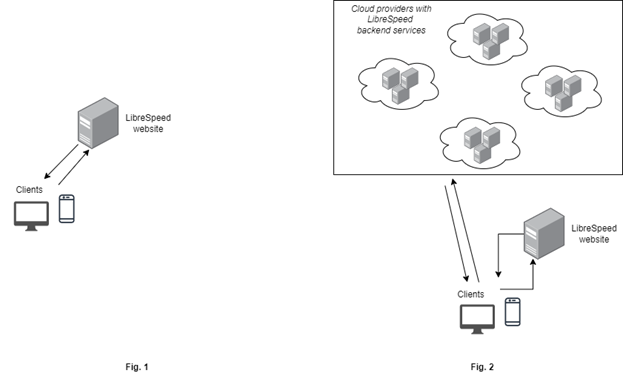
\includegraphics[width=\textwidth]{1-schema}
\end{minipage}
\end{center}

When the user wants to measure the latency and/or network speed, eventually they go to the LibreSpeed website, which shows a basic frontend. This portal loads a JavaScript file that triggers a function to load the available backend servers, which are provided in a JSON format directly into the index file of the frontend itself.

\begin{center}
\begin{minipage}{12cm}
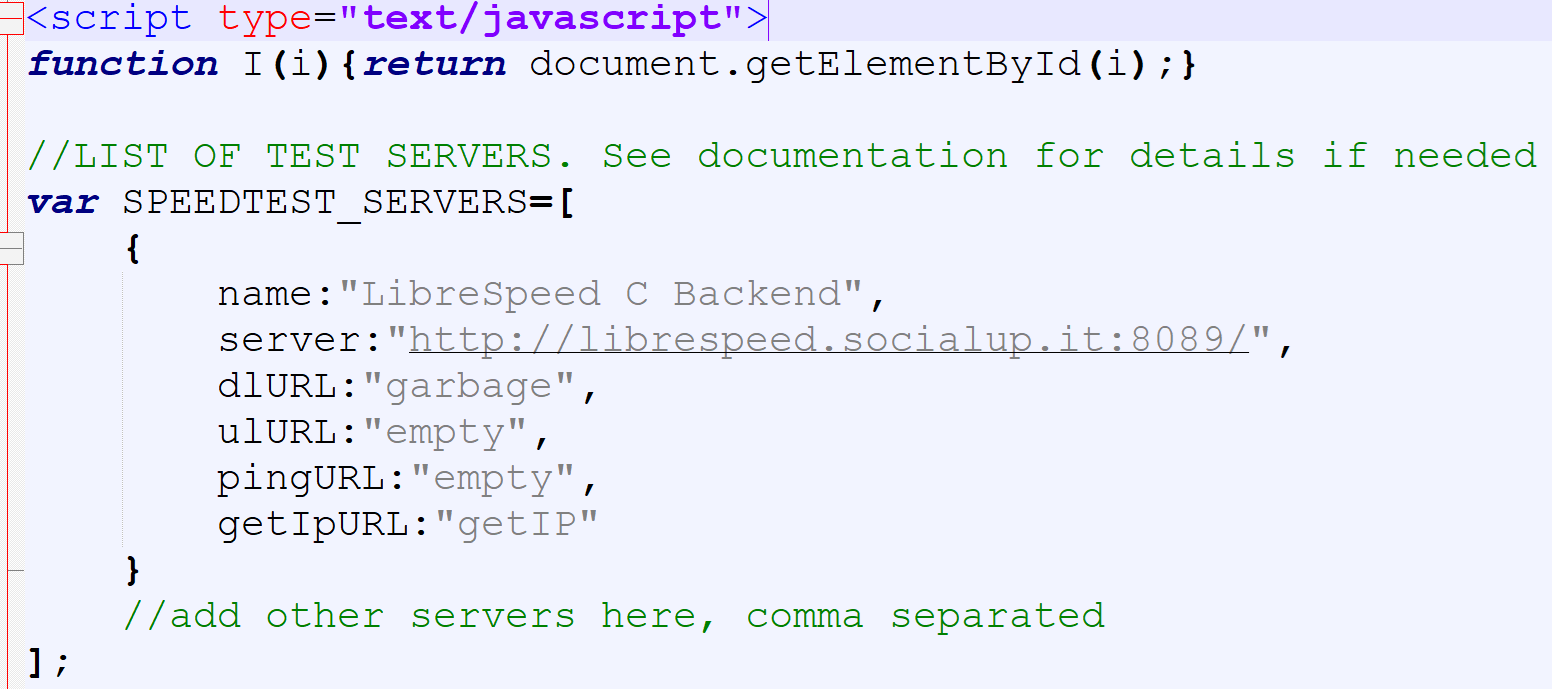
\includegraphics[width=\textwidth]{2-servers}
\end{minipage}
\end{center}
 
All server objects are made by some specific fields:
\begin{itemize}
\item \texttt{getIpURL} identifies the endpoint responsible for obtaining the client’s IP address. In the “advanced” backend it is possible to extend the precision of the information returned by calling an external API that will return the estimated distance of the client to the server. This is done to determine the closest server.
\item \texttt{name} is the visual label of the server, and it usually shows its city, country, and provider.
\item \texttt{pingURL} and ulURL identify the endpoint that works as a ping service. It usually has an empty response, and it is used to check the status OK.
\item \texttt{server} is the URL of the server for the endpoints listed in the fields above.
\item \texttt{dlURL} identifies the endpoint that creates and downloads a random file, made by “garbage” data. Its size is less or equal to 100 MB and is needed to determine in a reasonable time the user network speed.
\end{itemize}

Once this JSON response is loaded, the front end starts to ping each server and analyze the HTTP status code, in order to exclude the unresponsive or unhealthy servers.
Backend services can be loaded in two different configurations:
\begin{itemize}
\item Standalone (fig. 1): with this mode the backend services are hosted under the same server and domain of the frontend. For this reason, the front end may be overloaded with requests if the service is used by several people. This can be a valid choice for anyone who wants to build a personal speed test service.
\item Multiple points of the test (MPOT) (fig. 2): with this mode the backend services are hosted on one or more servers. This can be very useful in professional environments where performance, availability, and quality are essential.
\end{itemize}

Even though the chosen configuration may influence the backend services, it won’t affect the client, and the configuration will be totally imperceptible to the users.

\newpage
\section{Theory concepts}
\subsection{HTTP 1.1}
HTTP 1.1 is the latest version of the HTTP (hypertext transfer protocol) protocol that runs on top of the TCP/IP suite of protocols. Provides a faster and more reliable delivery of web pages and reduces web traffic. It is the natural successor to HTTP 1.0 and was developed by the Internet Engineering Task Force (IETF), including the inventor creator of the World Wide Web (WWW), Sir Tim Berners-Lee.
Instead of opening and closing a connection for every request, HTTP 1.1 provides the concept of a persistent connection. Is a simple but powerful concept, that allows multiple requests to be re-used or batched, or pipelined to an output buffer. The underlying TCP layer puts multiple requests into one TCP segment that gets forwarded to the IP layer for packet transmission. This improvement reduces dramatically the number of requests and increases performance for the user. In addition to these new functionalities, pages can be packed on the server-side and unpacked by the clients, saving amounts of data.
Another advantage of this new version of HTTP is the fact that multiple domain names could same IP address, also known as virtual hosting.

\begin{center}
\begin{minipage}{8cm}
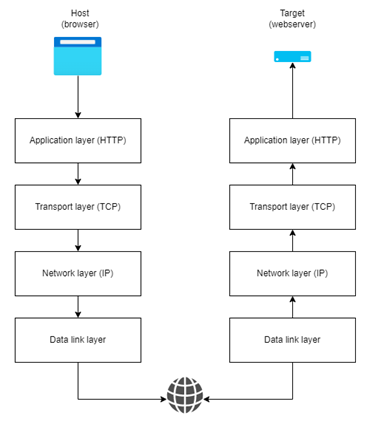
\includegraphics[width=\textwidth]{3-http}
\end{minipage}
\end{center}

When a client requests a resource to a server using a browser, some protocols are used to reach services and transport data through the Internet:
The application layer provides applications with data exchange. Its protocols include FTP, HTTP, POP3, and SMTP. At this layer, the payload is the actual application data.
The transport layer is responsible for maintaining end-to-end communications across the network. TCP handles communications between hosts and provides flow control.
The network layer deals with packets and connects networks to transport packets across network boundaries.
The data link layer is responsible for transferring data between nodes on a network across the physical layer.

\newpage
\section{Libre Speed C Backend}
\subsection{Introduction}
Even though C is a programming language that can do everything, developing web applications and web APIs can be particularly challenging, also because of the lack of easy-to-use libraries. The modern world of development is full of products and servers that can help the needs of everyone, from a static landing page to a complex web application that uses a database, cache, and load balancers. For example, Microsoft provides a wide range of languages and platforms regarding web development and services, and nowadays developing these kinds of projects can be very quick and easy, serving both HTTP and HTTPS requests.

\subsection{HTTPS limitation}
Regarding these protocols, for technical reasons, I decided to provide, at least in the initial phase, support only for HTTP requests, but since HTTPS is vital in terms of security I installed and configured in my server a reverse proxy (Apache2) that will serve and route HTTPS requests. This step is completely invisible to final users. In the future development, I will provide native support for HTTPS requests directly in the server, using some libraries to handle certificates and encryption.

\subsection{Demo and local testing}
The project is fully-working and available in my personal website. \href{https://speedtest.sergiomeloni.com}{speedtest.sergiomeloni.com}. The VM (Virtual Machine) is located in Germany and is currently hosted by Hetzner. Future planes will involve moving this resource from Hetzner to Microsoft Azure, in order to have better scalability, security and manageability. The operating system is Ubuntu Server 20.04.

The project can be compiled locally in any Linux-based distro, using the following command from the root folder:

\texttt{gcc -w -o server server.c -pthread}

If the command is successfully executed, you can run the server using the following command:

\texttt{./server}

The server will start listening on port \texttt{8089} (configurable in \texttt{settings.h} file) and the backend will be served. A sample-index welcome page is available for testing purposes at \href{http://localhost:8089/}{http://localhost:8089/}.

\subsection{The project}
The “LibreSpeed C Backend” is a project divided into several files, logically organized by function:

\begin{center}
\begin{minipage}{12cm}
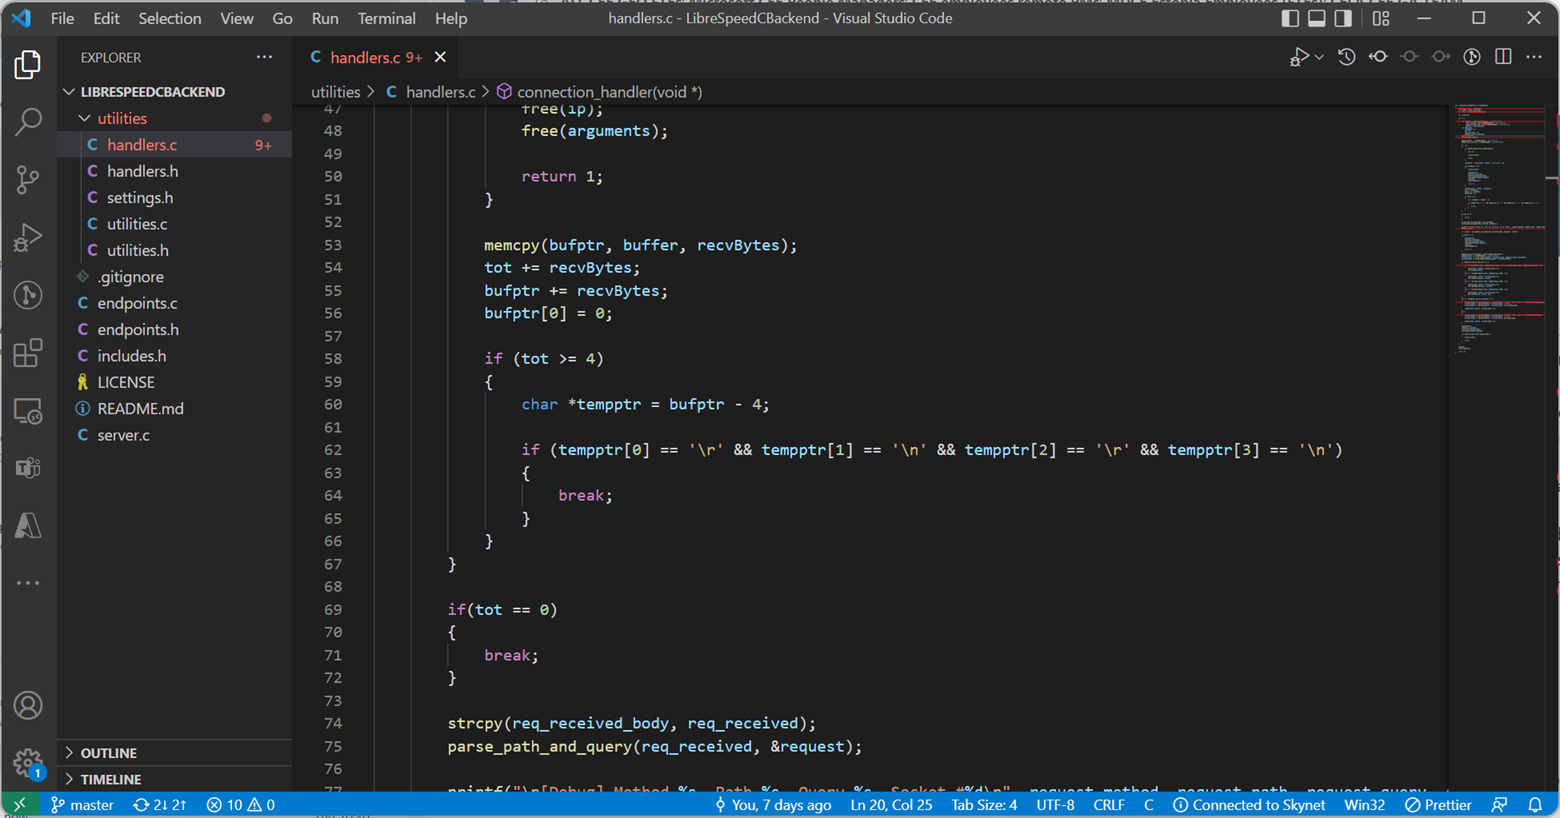
\includegraphics[width=\textwidth]{13-function}
\end{minipage}
\end{center}

Despite the name, this project is not just limited to backend endpoints but provides a full-working basic web server. Written in C, this server is extremely lightweight and can serve static files like documents, text files, HTML pages, etc. It is specifically designed for handling HTTP 1.1 requests and, in the first version, can serve 4 different endpoints, the ones needed by LibreSpeed to perform the speed test.

Since it works for HTTP 1.1, it relies on TCP sockets to create the concept of a persistent connection. Every time a new client connects to the server, a socket is opened and persisted (and eventually re-used) for the entire time until the client drops the connection or a new one is established. It relies also on threads to ensure a fluid and positive experience for multiple users at a time since one of the key functions of a speed test is to be usable by as many users as possible.

\subsection{Server code and architecture view}
\subsubsection{Server}
The entry point of the server is encapsulated in the server.c file, where an infinite loop in combination with the accept() function is responsible for assigning a socket and creating a thread that will handle all the server core functions. At this stage, the IP of the client is calculated from the socket itself. This is just one of the many functions written in the utilities.c file used to store all the most used functions of this server.

\subsubsection{Handler}
The core file of the server is represented by \texttt{handlers.c}, which contains the handler associated with the thread. With an infinite loop, the socket is actively listening, waiting for some bytes to read. These bytes should represent, in our case, an HTTP request, that will have this format, according to the related RFC.
A request message from a client to a server includes, within the first line of that message, the method to be applied to the resource, the identifier of the resource, and the protocol version in use and it has the following format:

\begin{center}
\begin{minipage}{8cm}
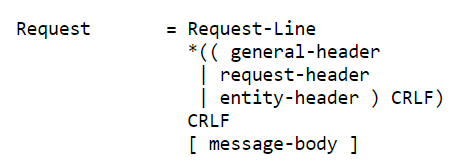
\includegraphics[width=\textwidth]{7-format}
\end{minipage}
\end{center}

The request-line always begins with a method, following the request URI, the protocol version, and an ending token, CRLF. All these elements are separated by the space character (SP).
The method indicates what should be performed on the URI, and the available methods supported by LibreSpeed C Backend Server are the following:
\begin{itemize}
\item POST
\item GET
\item OPTIONS
\end{itemize}

Currently, the server has a check to determine if a specific endpoint has been called with a specific method, in order to deny requests (and reply with a 405-status error) to unsupported methods.
The request URI identifies the path of the resource we are calling and based on that we can make decisions on which action should be called. At the current state of the art, all the possible actions are mocked and not served dynamically. One of the possible future developments will be serving dynamic content based on the provided URI, looking into a specific folder (a.k.a. document root).

During this stage, I keep going reading bytes until we reach the end of the request.
For every iteration in the cycle, I always check if the socket is still open, because a client may eventually close the connection unexpectedly. If it is the case, I will provide to free all the memory I allocated previously, because C does not come with a garbage collector.
Once the request has been read, I parse it using the function parse\_path\_and\_query(), sending it the raw bytes and a struct that will contain all the fields of the HTTP request, such as query, path, and method. In this phase, I divide the request by tokens splitting the entire string by a new line character. In this way, I will have a list of lines to easily handle operations and I can also save the eventual parameters that come into the query string.
Now that I have collected the method, path, and query I can start reading the eventual body of the request. To do that, I simply look in the raw request for the presence of the Content-Length property in the header. In case of problems or when the socket is closed, I return an error code and I immediately free the allocated memory and interrupt the thread.
After reading the body I will check the existence of the endpoint using the check\_endpoint() function, which simply looks for correspondence in the endpoint list (array of pre-filled paths) and returns a status code that may vary in case the endpoint is found or is not found or is found but with a not allowed method.
The following phase represents the first step in writing the response: the write\_response() function is responsible for setting the status code based on the result of the previous function: we will have a 200 for OK, 404 for “not found” and 405 for “method not allowed”.
After these parses, checks, and common stuff, there is the core of the endpoint selection: if the path does not exists or we received a not supported method we will reply with the related error message and a status code, otherwise, we can call the specific endpoint function.

\subsubsection{Utilities}
An important design decision made in my project has been separating the utility functions to the core files in order to logically maintain order.
In the file \texttt{utilities.c} under the utility folder I put various functions, and below there is an exhaustive list of them:

\begin{itemize}
\item \texttt{is\_numeric()} is a simple functions that takes in a string (\texttt{char *}) and return an \texttt{integer} value stating whether the input is a number or not. It is used, for example, to determine the number of chunks and convert it into a real number.
\item \texttt{get\_random\_bytes()} is a function that takes in a variable number of bytes and a \texttt{uint8\_t} pointer array and generates random bytes. Those values are stored in the input array. It is used in the \texttt{garbage} API to provide the user with a random file to download in order to determine the speed of download bandwidth.
\item \texttt{write\_common\_headers()} is a function that simply writes some common and repeated headers like the server name.
\item \texttt{write\_reponse()} is a function used to manage the status code of the response. Takes in an \texttt{integer} parameter representing the status code of the page (e.g. not found, OK, method not allowed, etc.) and writes the response in the HTTP headers.
\item \texttt{parse\_query\_params()} is a core function called in \texttt{handlers.c} main file. It is used, alongside with \texttt{parse\_path\_and\_query()} function to parse HTTP requests headers and save those informations into a struct passed as an input parameter. It is necessary and controls the correct flow of the program.
\item \texttt{get\_param\_exists()} is a function that takes in a string representing a query string parameter and returns a status code whether it has been passed to the request or not.
\item \texttt{get\_param\_value()} is a function that takes in a string representing a query string parameter and returns the value of the parameter passed to the request. It returns a \texttt{NULL} value if the parameter does not exist.
\item \texttt{get\_headers\_and\_body()} is again a core function of the program which lives in the \texttt{handlers.c} file. it is used to store in a memory buffer the content of the header and an optional body, in order for the program to process those values later during the execution.
\item \texttt{check\_endpoint()} is a function that verifies the existence of the endpoint in the array of the endpoints.
\item \texttt{check\_socket\_still\_open()} is an important function and checks whether the socket is not opened anymore. This function has been very important and the lack of it caused many memory leak problems, due to the infinite loops that were trying to receive bytes from an already closed connection.
\end{itemize}

\subsection{Endpoints}
This is the part of the server where the core path functions are defined. Here we can find the endpoints that define LibreSpeed C Backend, also called APIs. As already mentioned, I mocked functionality since the server can serve only static content.
What I currently have done is create four main functions, one for each endpoint.

\subsubsection{\texttt{/index} [GET]}
This is the basic and most simple endpoint: it does nothing than writing a message to a video that represents the index page (the default document). Ideally, someone can call the server URL and see this friendly message welcoming. Currently a request with a blank path or the root path “/” will be redirected to the index.

\subsubsection{\texttt{/empty} [GET, POST]}
As the name may suggest, this endpoint does nothing but show a blank page with no content. It is used to check two different speed test behaviors:”
\begin{itemize}
\item When the client sends some requests to the empty API. In this case, replies with an HTTP header and an empty body. It is required for the ping test, and the first time it starts, it will open a persistent connection. Once it is successfully opened, the client calls more time this API and since both request and response are very tiny and will be served on a single packet, the time spent in receiving the response is a round trip time.
\item And it is used for the upload phase too. The client generates and sends 20 MB of random data and sends them to the empty API using a POST method. This phase is necessary to determine the upload speed of the client.
\end{itemize}

\subsubsection{\texttt{/garbage} [GET]}
This function is used to generate and download a random file of a variable dimension. Based on some parameters sent with query string, we first determine how many chunks we want and then we send back as a response several bytes that correspond to the number of chunks multiplied by 1024.
An important note is that the client opens at the same time six parallel connections in order to saturate the bandwidth. This is required to have the maximum accuracy in determining the network download speed.

\subsubsection{\texttt{/getIP} [GET]}
This function is used to get the IP address of the client and shown on the homepage during the speed test.
Since I am using a reverse proxy to server HTTPS requests, I faced the problem that all the requests came from 127.0.0.1, the localhost. That is because the proxy was handling all the requests to decrypt them and was passing them to the server. To solve this problem I started getting the client IP from a special header called X-Forwarded-For.

\newpage
\section{Detecting and debugging problems}
After the development phase was finished, the Virtual Machine in the Microsoft Azure cloud has been set up to serve the APIs. During this time I monitored the status of the service and the general performances with \texttt{HTOP} command, which allowed me to have a minimal-UI interactive system monitor designed for Unix systems.

\begin{center}
\begin{minipage}{12cm}
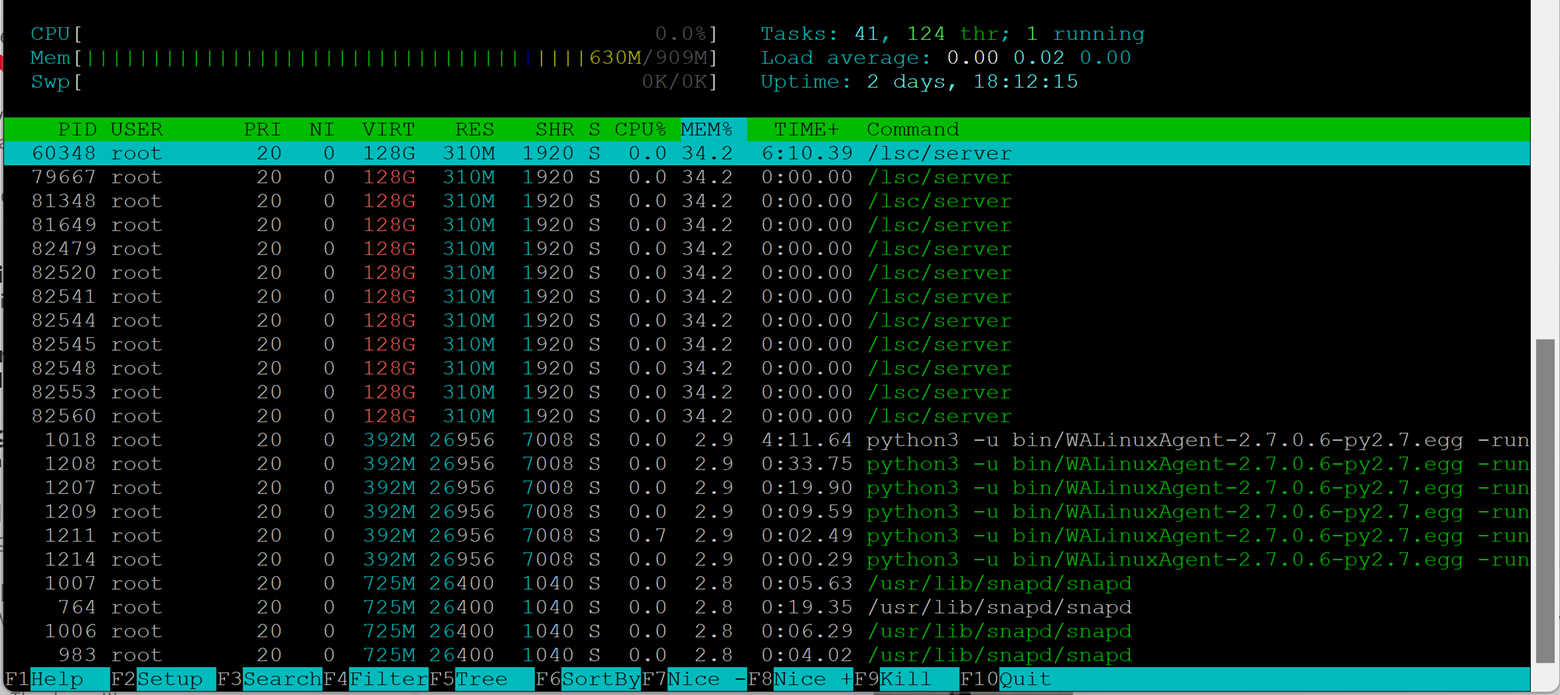
\includegraphics[width=\textwidth]{10-meml-1}
\end{minipage}
\end{center}

With this powerful tool after some time what caught my attention was the fact that the server was using an incredible amount of memory. In order to figure out what caused this problem, I decided to install and use another tool particularly useful in these situations.

\subsection{Valgrind}
Valgrind is an open-source framework for dynamic analysis. It is mainly used for detecting memory issues and threading bugs, and it includes a variety of tools like:
\begin{itemize}
\item memory error detector
\item thread error detector
\item cache and branch-prediction profiler
\item call-graph generating cache
\item heap profilers
\end{itemize}

and it runs on a variety of platforms and Unix-based OSs. Using this tool I have been able to analyze one hour of incoming traffic and detect some issues like the one below:

\begin{center}
\begin{minipage}{12cm}
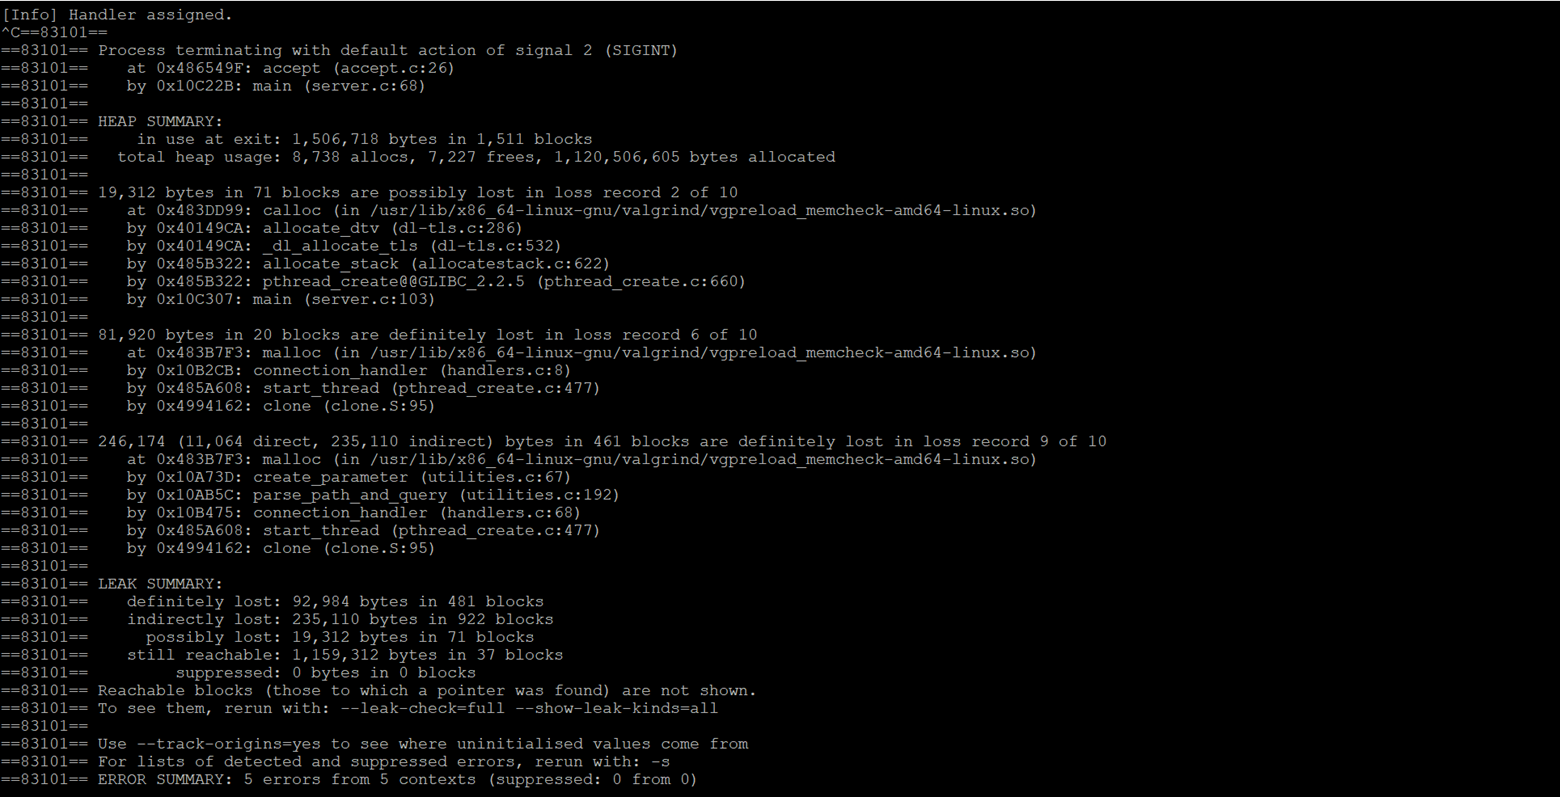
\includegraphics[width=\textwidth]{12-meml-3}
\end{minipage}
\end{center}

In this example, I have been able to identify a problem happening on the heap about some memory allocation that I forgot to deallocate after using. In particular, to store incoming query string parameters I was using a linked list in order to save some memory. Valgrind raised some red flags pointing out that when I create the memory element inside the \texttt{create\_parameter()} function, I was not using \texttt{free()} at the end of the process, causing a rapid heap filling.

One other problem I have been able to solve with this tool was when I noticed a 100\% usage of the CPU. In that case, Valgrind helped me understand that the issue was caused by \texttt{recv()} function: in one infinite loop I was trying to read some bytes from an already closed socket. That did not cause any kind of termination, but since the exit condition of the loop was determined by the CRLF character, this caused a never-ending process, resulting in high CPU usage.

\newpage
\section{License}
The License of use of LibreSpeed C Backend states under the \texttt{GNU GPL v3.0}. This Type of license says that "nobody should be restricted by the software they use". This one, in particular, has four important points that should be respected:
\begin{itemize}
\item The freedom to use the software for any purpose.
\item The freedom to change the software to suit your needs.
\item The freedom to share the software with your friends and neighbors.
\item The freedom to share the changes you make.
\end{itemize}
GPL v3 act as a strong copyleft license, meaning that any kind of modification, addition and copy of the original code must be released under the GPL v3 too. In other words cloning, forking, making major or minor code is always possible as well as contributing, but the new version should be placed and distributed under the same type of license.

\subsection{Requirements}
The license terms of GPL v2 and GPL v3 are similar. They require developers to:
\begin{itemize}
\item Include a copy of the full license text.
\item State all significant changes made to the original software.
\item Make available the source code when you distribute any binaries based on the licensed work.
\item Include a copy of the original copyright notice.
\end{itemize}

Additionally, the GPL v3 license states that people that includes the code as part of a consumer devices has the obligation to include any relevant installation information necessary in order to update, reinstall and use the software.

\subsection{Using the Licensed Code}
The GPL v3 license allows developers to:

\begin{itemize}
\item Use the code for commercial purposes: Like GPL v2, GPL v3 has no really impositions on how the code is used for, hence the commercial use is permitted.
\item Change the code: Users can change the code as their own, but if they re-distribute these modifications, they are also required to release these updates (in form of source code) under the GPL v3 license.
\item Distribute copies or modifications of the code: As long as these modifications are also released under the GPL v3 license, they can be distributed to others.
\item Place warranty: Distributors of the original code can (but not obliged to) offer their warranty on the licensed software.
\end{itemize}

Like v2, GPL v3 does not allow users to sublicense the code. In other words, it is not possible to "rework" the code and then close those changes off to the public. The "open source-ness" of the original code follows any update or addition.

\newpage
\section{Links and other material}
In this section and the below subsections, I will put all the external resources, websites, and material I used to prepare this project relation.

\begin{enumerate}
\item \href{https://www.fdossena.com}{Federico Dossena personal Website}.
\item \href{https://github.com/librespeed}{LibreSpeed Official GitHub repo}.
\item \href{https://www.librespeed.org/}{LibreSpeed Official Website}.
\item \href{https://github.com/sergiusxp/LibreSpeedCBackend}{LibreSpeed C Backend Official GitHub repo}.
\item \href{https://speedtest.sergiomeloni.com}{LibreSpeed C Backend Official website}.
\item \href{https://speedtest.net}{speedtest.net}
\item \href{https://fast.com}{fast.com}
\item \href{https://speedof.me}{speedof.me}
\item \href{https://testmy.net}{testmy.net}
\item \href{https://www.gnu.org/licenses/quick-guide-gplv3.en.html}{Quick guide to GNU GPL license}.
\end{enumerate}

\end{document}
